\documentclass[letter,11pt]{article}
\usepackage[pdftex]{graphicx}
\usepackage{float}
\begin{document}
	\begin{center}
		\Large\textbf{CSCI 567-Machine Learning Assignment-2}
	\end{center}
	
	\section{Naive Bayes}
	\subsection{Priors and Conditionals}
	Priors of each dependent variable is:
	$$P(no) = \sum_{password} P(no|password)P(password)$$
	$$P(no) = P(password = 240)P(no|password = 240) + P(password = 343)P(no|password =343)$$
	$$P(no) = \frac{8}{9}$$

	$$P(yes) = \sum_{password} P(yes|password)P(password) = \frac{1}{9}$$
	Let's define each $x_i:$ Number $i$ is in password\\
	$P(x_0|y = no) = 0.5$   \hspace{10mm}	$P(x_0|y = yes) = 0.5$\\
	$P(x_1|y = no) = 0.01$\hspace{9mm}	$P(x_1|y = yes) = 0.5$\\
	$P(x_2|y = no) = 0.5$\hspace{10mm}	$P(x_2|y = yes) = 0.5$\\
	$P(x_3|y = no) = 0.5$\hspace{10mm}	$P(x_3|y = yes) = 0.5$\\
    $P(x_4|y = no) = 1$\hspace{12mm}	$P(x_4|y = yes) = 0.5$\\
    
	\subsection{Password 031}
	Let $N_{x_i}$ be the number of $i$'s in password.
	$$P(y|x) = \frac{P(x|y)P(y)}{P(x)}=\prod P(x|y)^{N_x}P(y)$$
	Two different class:
	$$P(yes|031) = \prod P(x_i|yes)^{N_{x_i}}P(yes) = P(x_0|yes)P(x_3|yes)P(x_1|yes)P(yes)$$
	$$P(yes|031) = 0.5*0.5*0.5*\frac{1}{9} = 0.0134$$
	$$P(no|031) = \prod P(x_i|no)^{N_{x_i}}P(no) = P(x_0|no)P(x_3|no)P(x_1|no)P(no)$$
	$$P(no|031) = 0.5*0.5*0.01*\frac{8}{9} = 0.0022$$	
	
	Since $P(yes|031)$ is larger than $P(no|031)$, Naive Bayes Classifier will classify $031$ password as "Yes".
	
	\subsection{Logistic Regression is Discriminative Version of Naive Bayes}
 
	\hspace{7mm}Logistic Regression and Naive Bayes are both classifiers. Naive Bayes Classifier aims to model the joint probability $P(x,y)$ and thus maximizes the joint likelihood $\sum log P(x_n,y_n)$.\\
	
	Both Logistic Regression and NBC are linear classifiers that decides on the decision boundary between classes. Naive Bayes' decision boundary is set by $w_0 + \sum_{k}z_kw_k$ and Logistic Regression's decision boundary is $w_0 + \sum_{k}w_kx_k$.\\
	
	
	To get these decision boundaries, Naive Bayes and other Generative models, model $P(x|y)$ and $P(y)$ and Naive Bayes uses the Bayes' rule to get the joint probability.
	$$ f(x) = \arg\max_y P(x|y)P(y)$$
	
	On the other hand, Logistic Regression requires only specifying a model for the conditional distribution $P(y|x)$ and maximizes this conditional likelihood $\sum_{n}logP(y_n|x_n).$\\
	
	Logistic regression sets all the weights together such that the linear decision function tends to be high for positive classes and low for negative.
	
	$$f(x) = \arg\max_y Py|x)$$
	
	\subsection{Assumption of Naive Bayes Classifier}
	
	Naive Bayes Classifier sets each features weight independently, based on how much it correlates with the label. The Naive Bayes classifier does this
	by making a conditional independence assumption that dramatically reduces the
	number of parameters to be estimated when modeling P(X|Y).\\
	
	Because this conditional independence assumption is violated when there is correlated features, Logistic Regression outperforms Naive Bayes Classifier in most cases, which makes it more generic then NBC. 
	
	\section{Generative Model and Discriminative Model}
	\subsection{MLE of Parameters}	
	$$P(D_i|\Pi,\mu_0,\mu_1,S_0,S_1) = [(1-\Pi) \frac{1}{\sqrt{2\pi}S_0}\exp(-\frac{1}{2S_0^2}(x_i-\mu_0)^2))^{t_{n0}}$$$$((\Pi)\frac{1}{\sqrt{2\pi}S_1}\exp(-\frac{1}{2S_1^2}(x_i-\mu_1)^2))^{t_{n1}}]$$
	
	$$logP(D|\Pi,\mu_0,\mu_1,S_0,S_1) = \sum_{n=1}^{N}t_{n0}[log(1-\Pi)-\frac{1}{2}log(2\pi) - logS_0 - \frac{1}{2S_0}(x_n-\mu_0)^2] +$$ $$\sum_{n=1}^{N}t_{n1}[log\Pi - \frac{1}{2}log(2\pi)-logS_1 - \frac{1}{2S_1}(x_n-\mu_1)^2]$$
	
	Derivative for $\Pi$:
	$$\frac{\partial logP(D|\Pi,\mu_0,\mu_1,S_0,S_1)}{\partial\pi} = N_1\frac{1}{\Pi} - N_0\frac{1}{1-\Pi} = 0$$
	$$\Pi = \frac{N_1}{N_0 + N_1}$$
	
	Derivative for $\mu_0$ and $\mu_1$:
	$$\frac{\partial logP(D|\Pi,\mu_0,\mu_1,S_0,S_1)}{\partial\mu_0} = \frac{\sum t_{n0}x_n}{S_0} - \frac{N_0\mu_0}{S_0} = 0$$
	$$\mu_0 = \frac{\sum t_{n0}x_i}{N_0}$$
	$$\mu_1 = \frac{\sum t_{n1}x_i}{N_1}$$
	
	Derivative for $S_0$ and $S_1$:
	$$\frac{\partial logP(D|\Pi,\mu_0,\mu_1,S_0,S_1)}{\partial S_0} = -\frac{N_0}{S_0} + \frac{1}{2S_0^2}\sum t_{n0}(x_n-\mu_0)^2 = 0$$
	$$S_0 = \frac{\sum t_{n0}(x_n-\mu_0)^2}{N_0}$$
	$$S_1 = \frac{\sum t_{n1}(x_n-\mu_1)^2}{N_1}$$	
	
	\subsection{Posterior Probability}
	
	$$p(y = 1|x,\pi,\mu_0,\mu_1,S_0,S_1) = \frac{p(y=1|\pi)p(x|y,\mu_1,S_1)}{p(y=1|\pi)p(x|\mu_1,S_1)+p(y=0|\pi)p(x|\mu_0,S_0)}$$
	
	This has the form of:
	$$P(y = 1|x) = \frac{P(y=1)p(x|y=1)}{P(y=1)p(x|y=1)+p(y=0)p(x|y=0)}$$
	Divide both nominator and denominator by nominator:
	$$ = \frac{1}{1 + \frac{p(y=0)p(x|y=0)}{P(y=1)p(x|y=1)}} = \frac{1}{1 + exp(log \frac{p(y=0)p(x|y=0)}{P(y=1)p(x|y=1)})}$$
	$$ = \frac{1}{1 + exp(log \frac{p(y=0)}{p(y=1)}+ \sum_{n}log\frac{p(x_n|y=0)}{p(x_n|y=1)})}$$
	Given the parameters in the question and $S_0 = S_1 = S $:
	$$\sum_{n}log\frac{p(x_n|y=0)}{p(x_n|y=1)} = \sum log \frac{\frac{1}{\sqrt{2\pi}S_n}\exp-(\frac{(x_n - \mu_{n0})^2}{2S_n^2})}{\frac{1}{\sqrt{2\pi}S_n}\exp -(\frac{(x_n - \mu_{n1})^2}{2S_n^2})} = \sum (\frac{\mu_{n0}-\mu_{n1}}{S_n^2}x_n + \frac{\mu_{n1}^2-\mu_{n0}^2}{2S_n^2})$$
	
	Put in equation:
	$$P(y = 1|x) = \frac{1}{1 + \exp(log\frac{1-\pi}{\pi} + \sum_{n}(\frac{\mu_{n0}-\mu_{n1}}{S_n^2}x_n + \frac{\mu_{n1}^2-\mu_{n0}^2}{2S_n^2}))}$$
	
	In this case:
	$$w_0 = log \frac{1-\pi}{\pi} + \sum_{n}\frac{\mu_{n1}^2 - \mu_{n0}^2}{2S_i^2}$$
	$$w_i = \frac{\mu_{i0} - \mu_{i1}}{S_i^2}$$
	
	\subsection{Poisson Mixture Distribution}
	Starting from this:
		$$P(y = 1|x)  = \frac{1}{1 + exp(log \frac{p(y=0)}{p(y=1)}+ \sum_{n}log\frac{p(x_n|y=0)}{p(x_n|y=1)})} = \frac{1}{1 + exp(log \frac{1-\pi}{\pi} + \sum_{i} log \frac{\exp(-\lambda_{0i})\lambda_{0i}^{x_i}}{\exp(-\lambda_{1i})\lambda_{1i}^{x_i}})}$$
		$$ = \frac{1}{1 + exp(log \frac{1-\pi}{\pi} + \sum_{i}(\lambda_{1i} - \lambda_{0i})x_i(log \lambda_{0i} - log \lambda_{1i})}$$
		$$ w_0 = log \frac{1-\pi}{\pi}$$
		$$ w_i = (\lambda_{1i} - \lambda_{0i})(log \lambda_{0i}0 - log \lambda_{1i})$$
		
		
		
		\section{Multinomial Logistic Regression}
		
		\section{Programming Questions}
		\begin{center}
			\begin{tabular}{|c| c |c |c|} 
				\hline
				Method & Data Type & Training Acc & Test Acc \\ [0.5ex] 
				\hline
				Batch Gradient & raw & 0.8692 & 0.8817 \\ 
				\hline
				Batch Gradient & standardized & 0.9300 & 0.9261 \\
				\hline
				Newton's Method & raw & 0.8935 & 0.8922 \\
				\hline
				Newton's Method & standardized & 0.8935 & 0.8922 \\
				\hline
				glmfit & raw & 0.9357 & 0.9265 \\
				\hline
			    glmfit & standardized & 0.9357 & 0.9265 \\
				\hline
			\end{tabular}
		\end{center}
%	\begin{figure}[H]%                 use [hb] only if necceccary!
%	\centering
%	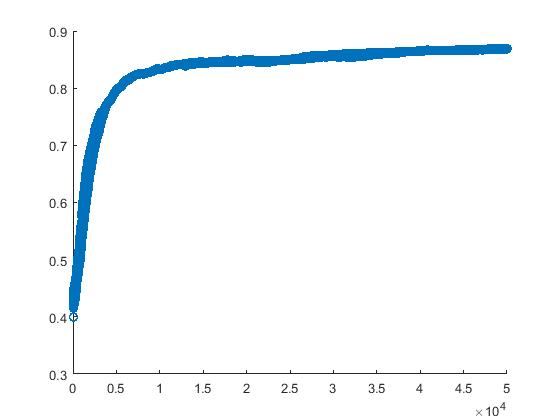
\includegraphics[width=9cm]{C:/Users/okazk_000/Desktop/Spring 2016/CSCI 567/HW2/hw2/accTrainGrad.jpg}
%	\caption{Batch Gradient over 50.000 iterations}
%	\label{fig:test}
%	\end{figure}
	\subsubsection{Chosen 20 Features}
	The feature IDs chosen according to Mutual Information values:\\
	$[52,53,56,21,55,7,16,57,25,19,24,5,27,17,3,26,23,6,11,2]$
	
	Using these 20 features on glmfit function: 
	Training accuracy = $0.8914$ and Testing Accuracy = $0.8926$
	
	\subsection{Generative Model and Discriminative Model}
	\subsubsection{MLE Parameters When Variances Are Independent}
	
	Component Proportions = ([0.2941,0.2679,0.4379])\\
	$\mu$ Parameters = ([1.538,0.0354; -1.593,1.596; -1.486,-1.408])\\
	$\Sigma$ Parameters  =\\
	First Component \hspace{15mm} Second Component \hspace{15mm} Third Component
	0.9988    0.0102 \hspace{25mm}  1.0197   -0.4525 \hspace{25mm}      1.0280    0.5110
    0.0102    3.9734  \hspace{25mm} -0.4525    1.0105 \hspace{24mm}      0.5110    1.1234\\
    Testing Accuracy = 0.9007
    
    \subsubsection{MLE Parameters When Variances Are Equal}
	Component Proportions = ([0.293,0.275,0.430])\\
	$\mu$ Parameters = ([1.549,0.0435;-1.759,-0.739;-1.385,0.0282])\\
	$\Sigma$ Parameters  =\\
	0.977 -0.004\\
	 -0.004 3.331\\
	Testing Accuracy = 0.7600
	
	\subsubsection{Multinomial Logistic Model}
	Testing Accuracy = 0.8846
	
	\subsubsection{Plot and Analysis}	
		 
		 We can see that the the best decision boundaries are given by Gaussian Mixture Model with different variance. And the worst one is given by Gaussian Mixture Model with same variance.\\
		 
		 
		 It is obvious that variances of three Gaussian models are different from each other. Even though green and blue colored data points have a similar variance, red colored data points' distribution has much larger variance. Since we made the same variance assumption in second model, it is reasonable to get not a very good decision boundary.\\
		 
		 On the other hand, logistic regression has made a very good classification and draw a good decision boundary between classes even though it couldn't use the advantage of being nonlinear as different variance Gaussian Mixture Model did.
		 
		 
		 
	 \subsubsection{Subset Training Data}
	 3 plots below shows the testing accuracy w.r.t. training data sizes for three models.


	\subsection{Practical Logistic Regression on Toy Data}
	\subsubsection{Discretization}
	The best model is chosen according to the best cross-validation accuracy. Leave one out technique is used.
		\begin{center}
			\begin{tabular}{|c| c |c |c | c |} 
				\hline
				Data & Best Discretization & Training Acc & Test Acc & Heldout Acc\\ [0.5ex] 
				\hline
				1 & $16^2$ & 0.9950 & 0.9737 & 0.9775 \\ 
				\hline
				2 & $16^2$ & 0.9975 & 0.9949 & 0.9925 \\
				\hline
				3 & $16^2$ & 1 & 0.9950 & 1 \\
				\hline
				4 & $4^2$ & 0.9800 & 0.9539 & 0.9675\\
				\hline
			\end{tabular}
		\end{center}	 
	\subsubsection{$\l$2 norm regularization)}
	For Data1:		
		\begin{center}
			\begin{tabular}{|c| c |c |c | c |} 
				\hline
				Type & $\lambda = 1$ &  $\lambda = 0.1$  &  $\lambda = 0.01$  &  $\lambda = 0.001$ \\ [0.5ex] 
				\hline
				Training Accuracy & 0.9700 & 0.9750 & 0.9775 & 0.9775 \\ 
				\hline
				Heldout Accuracy & 0.9700 & 0.9700 & 0.9700 & 0.9700 \\
				\hline
				Testing Accuracy & 0.9559 & 0.9583 & 0.9611 & 0.9612 \\
				\hline
			\end{tabular}
		\end{center}
	For Data2:		
	\begin{center}
		\begin{tabular}{|c| c |c |c | c |} 
			\hline
			Type & $\lambda = 1$ &  $\lambda = 0.1$  &  $\lambda = 0.01$  &  $\lambda = 0.001$ \\ [0.5ex] 
			\hline
			Training Accuracy & 0.9850 & 0.9850 & 0.9825 & 0.9825 \\ 
			\hline
			Heldout Accuracy & 0.9825 & 0.9825 & 0.9800 & 0.9800 \\
			\hline
			Testing Accuracy & 0.9833 & 0.9871 & 0.9915 & 0.9915 \\
			\hline
		\end{tabular}
	\end{center}
	For Data3:		
	\begin{center}
		\begin{tabular}{|c| c |c |c | c |} 
			\hline
			Type & $\lambda = 1$ &  $\lambda = 0.1$  &  $\lambda = 0.01$  &  $\lambda = 0.001$ \\ [0.5ex] 
			\hline
			Training Accuracy & 0.9800 & 0.9850 & 0.9900 & 0.9950 \\ 
			\hline
			Heldout Accuracy & 0.9800 & 0.9800 & 0.9800 & 0.9800 \\
			\hline
			Testing Accuracy & 0.9741 & 0.9760 & 0.9779 & 0.9783 \\
			\hline
		\end{tabular}
	\end{center}
	For Data4:		
	\begin{center}
		\begin{tabular}{|c| c |c |c | c |} 
			\hline
			Type & $\lambda = 1$ &  $\lambda = 0.1$  &  $\lambda = 0.01$  &  $\lambda = 0.001$ \\ [0.5ex] 
			\hline
			Training Accuracy & 0.9525 & 0.9800 & 0.9800 & 0.9825 \\ 
			\hline
			Heldout Accuracy & 0.9425 & 0.9675 & 0.9550 & 0.9625 \\
			\hline
			Testing Accuracy & 0.9425 & 0.9539 & 0.9520 & 0.9587 \\
			\hline
		\end{tabular}
	\end{center}
	\subsubsection{Visualization}
		For regularized terms; for Data2  $\lambda$ chosen as 1 and for Data3 $\lambda$ is chosen as 0.1.//
		For unregularized models for data2 and data3 are both $16^2$ discretizations.
		
		 
								
\end{document}